\chapter{جدول تقدّم التفاعل}\label{ch:g10:reaction-progress-table}

% ledger: use:NaN3-airbag
في حادث سيارة تنفجر وسادة من المقود وتمتلئ بالغاز في جزء من الثانية، قبل أن
يندفع رأس السائق إلى الأمام. والغاز يصنعه \omterm{def:g7:chemical-reactions:reaction}{تفاعل كيميائي}: شحنة صغيرة من جسم
صلب، هو أزيد الصوديوم في التصميم التقليدي، تتفكك إلى صوديوم ونيتروجين. وعلى
المهندس أن يضع من الجسم الصلب ما يكفي لملء الوسادة، لكن لا إلى حد أن تنفجر،
ولا يجوز أن يبقى أي \omterm{def:g7:chemical-reactions:reactant}{متفاعل} يؤذي الركاب. فكم من الجسم الصلب يعطي كم من الغاز؟
\omterm{def:g8:balanced-equations:equation}{المعادلة الموزونة} تعطي النسب؛ وهذا الفصل يحوّلها إلى أداة محاسبة تتبع كل
\omterm{def:g7:chemical-reactions:reactant}{متفاعل} وكل \omterm{def:g7:chemical-reactions:reactant}{ناتج} من بداية التفاعل إلى
نهايته.

\begin{recall}
\omterm{def:g8:balanced-equations:equation}{المعادلة الموزونة} تُبقي عدد \omterm{def:g7:atoms-and-molecules:atom}{ذرات} كل عنصر، والشحنة، واحدًا في الطرفين؛
ومعاملاتها تعطي النسب التي تتفاعل بها الأنواع (\cref{ch:g8:balanced-equations}).
\omterm{def:g10:the-mole:amount}{وكمية مادة} نوع هي $n = m/M$ لكتلة، و$n = V/V_m$ لغاز (مع
$V_m = \qty{24.1}{L/mol}$ عند \qty{20}{\celsius} والضغط الجوي
العادي) (\cref{ch:g10:the-mole})، و$n = c \times V$ \omterm{def:g6:solutions-and-solubility:solute}{لمذاب}
(\cref{ch:g10:concentration-and-dilution}).
\end{recall}

\begin{omfigure}
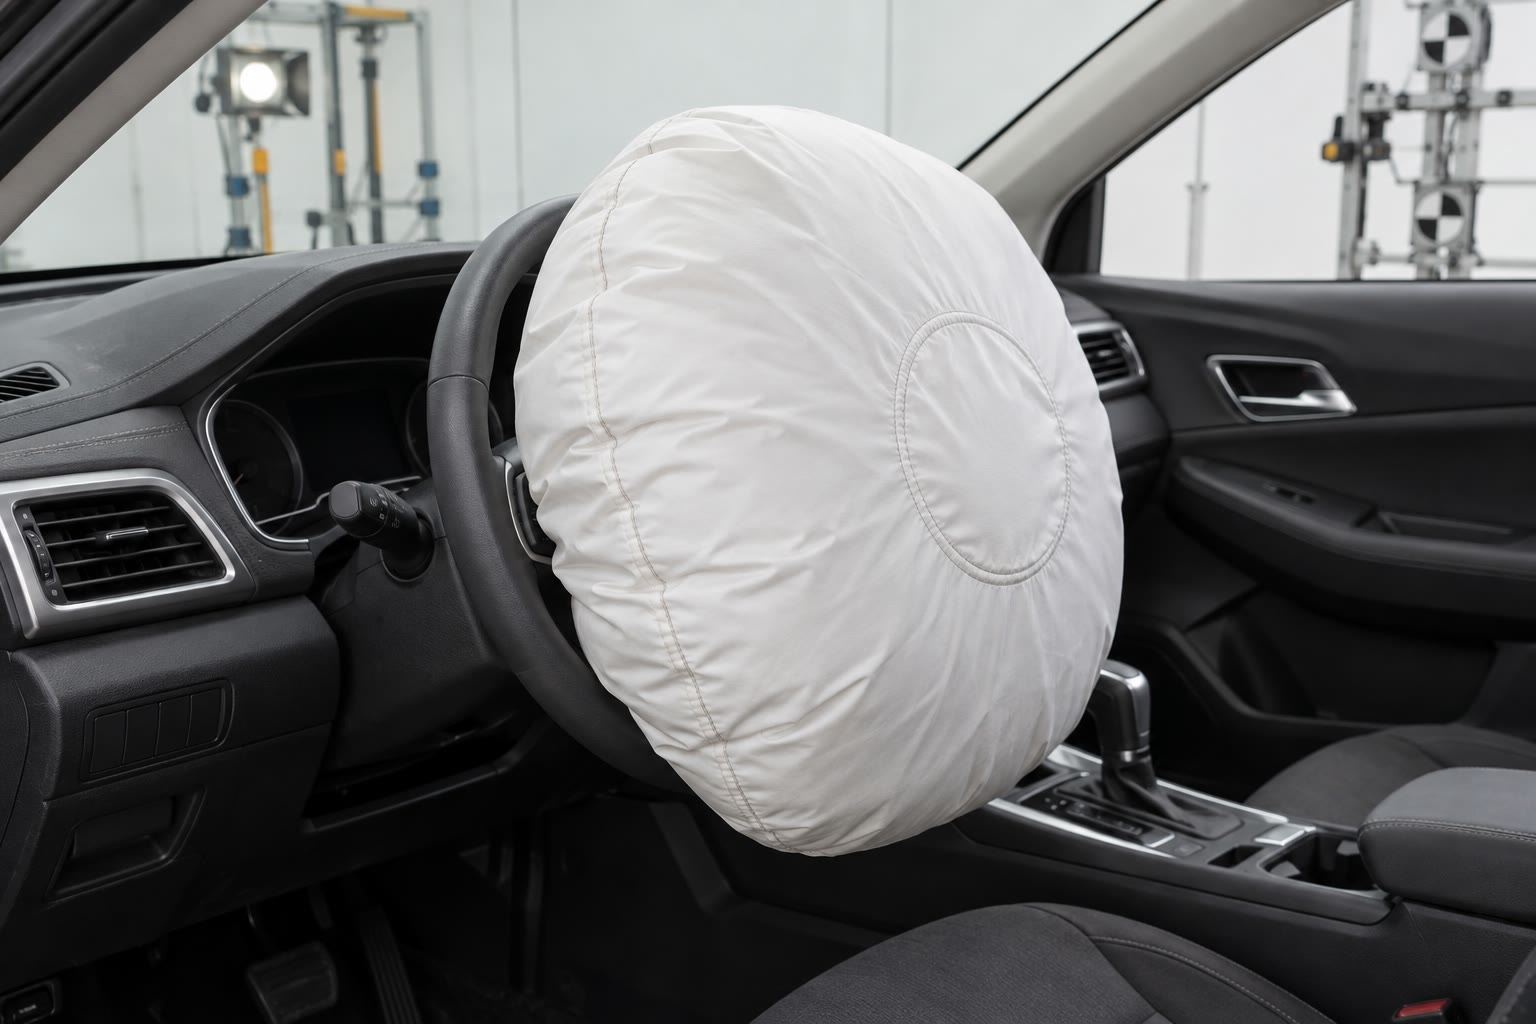
\includegraphics[width=0.5\linewidth]{images/book1/ai/g10-airbag.jpg}

{\small وسادة هوائية تمتلئ في جزء من الثانية، بالنيتروجين الذي يصنعه
تفاعل.}
\end{omfigure}

\section{وصف نظام كيميائي}

\begin{definition}[النظام الكيميائي والحالتان الابتدائية والنهائية]\label{def:g10:reaction-progress-table:system}
\emph{النظام الكيميائي}\index{نظام كيميائي} مجموع الأنواع الكيميائية
الموجودة في مكان معيّن (دورق، أو وسادة، أو خلية)، لكل منها كمية مادته وحالته
الفيزيائية. والنظام قبل بدء التفاعل هو \emph{الحالة الابتدائية}\index{حالة ابتدائية}؛
والنظام بعد توقف التفاعل هو \emph{الحالة
النهائية}\index{حالة نهائية}.
\end{definition}


\begin{example}[احتراق الميثان في وعاء مغلق]\label{ex:g10:reaction-progress-table:methane}
يحوي وعاء مغلق \qty{2.0}{mol} من الميثان و\qty{3.0}{mol} من
ثنائي الأكسجين؛ وتُطلق شرارة \omterm{def:g4:what-a-fire-needs:burning}{الاحتراق}
\ce{CH4 + 2O2 -> CO2 + 2H2O}. في \omterm{def:g10:reaction-progress-table:system}{الحالة الابتدائية} يحوي النظام
\qty{2.0}{mol} من \ce{CH4(g)} و\qty{3.0}{mol} من \ce{O2(g)} ولا
نواتج. فماذا في \omterm{def:g10:reaction-progress-table:system}{الحالة النهائية}؟ يجيب بقية الفصل عن ذلك.
\end{example}

\section{تقدّم التفاعل وجدول التقدّم}

\begin{definition}[تقدّم التفاعل، وجدول التقدّم]\label{def:g10:reaction-progress-table:extent}
\emph{تقدّم التفاعل}\index{تقدم التفاعل} $x$، \omterm{def:g10:the-mole:amount}{بالمول}، يعدّ كم مرة حدث
التفاعل، كما هو مكتوب في \omterm{def:g8:balanced-equations:equation}{المعادلة الموزونة}: فحين يكون التقدّم $x$ يكون نوع
معامله $\nu$ قد استُهلك (\omterm{def:g7:chemical-reactions:reactant}{متفاعل}) أو تكوّن (\omterm{def:g7:chemical-reactions:reactant}{ناتج}) بكمية
$\nu x$. و\emph{جدول التقدّم}\index{جدول التقدم} يعطي، تحت المعادلة، \omterm{def:g10:the-mole:amount}{كمية
مادة} كل نوع في \omterm{def:g10:reaction-progress-table:system}{الحالة الابتدائية}، وعند تقدّم $x$، وفي \omterm{def:g10:reaction-progress-table:system}{الحالة
النهائية}.
\end{definition}

\begin{method}[ملء جدول التقدّم]\label{met:g10:reaction-progress-table:fill}
\begin{enumerate}
  \item اكتب \omterm{def:g8:balanced-equations:equation}{المعادلة الموزونة} في السطر الأول.
  \item \omterm{def:g10:reaction-progress-table:system}{الحالة الابتدائية} ($x = 0$): اكتب تحتها الكمية الابتدائية لكل
        نوع.
  \item الحالة الوسيطة (التقدّم $x$): كل \omterm{def:g7:chemical-reactions:reactant}{متفاعل} معامله
        $\nu$ يصير $n_0 - \nu x$، وكل \omterm{def:g7:chemical-reactions:reactant}{ناتج} $n_0 + \nu x$.
  \item \omterm{def:g10:reaction-progress-table:system}{الحالة النهائية}: جد $x_{\max}$ (القسم التالي) وعوّضه في
        عبارات السطر الوسيط.
\end{enumerate}
\end{method}

\begin{omfigure}
\renewcommand{\arraystretch}{1.25}
\begin{tabular}{l|c|cccc}
\hline
المعادلة & & \ce{CH4} & $+$ \ce{2O2} & $\longleftarrow$ \ce{CO2} & $+$ \ce{2H2O} \\
\hline
الحالة & التقدّم (\si{mol}) & \multicolumn{4}{c}{كميات المادة (\si{mol})} \\
\hline
الابتدائية & $0$ & $2.0$ & $3.0$ & $0$ & $0$ \\
الوسيطة & $x$ & $2.0 - x$ & $3.0 - 2x$ & $x$ & $2x$ \\
النهائية & $x_{\max} = 1.5$ & $0.5$ & $0$ & $1.5$ & $3.0$ \\
\hline
\end{tabular}\par\medskip

{\small جدول تقدّم \omterm{def:g4:what-a-fire-needs:burning}{احتراق} الميثان في المثال. كل عمود يتبع نوعًا واحدًا؛ والمعاملان
2 لكل من \ce{O2} و\ce{H2O} يصيران
$2x$.}
\end{omfigure}

\section{المتفاعل المحدِّد والحالة النهائية}

\begin{definition}[المتفاعل المحدِّد، والتقدّم الأقصى، والتفاعل التام]\label{def:g10:reaction-progress-table:limiting}
يكون التفاعل \emph{تفاعلًا تامًا}\index{تفاعل تام} إذا لم يتوقف إلا حين يُستهلك
أحد متفاعلاته. وذلك \omterm{def:g7:chemical-reactions:reactant}{المتفاعل} هو \emph{المتفاعل المحدِّد}\index{متفاعل محدد}؛
\omterm{def:g7:chemical-reactions:reactant}{والمتفاعلات} الأخرى بزيادة. والتقدّم الذي ينفد عنده \omterm{def:g7:chemical-reactions:reactant}{المتفاعل} المحدِّد هو
\emph{التقدّم الأقصى}\index{تقدم أقصى} $x_{\max}$؛ \omterm{def:g10:reaction-progress-table:system}{والحالة النهائية} للتفاعل
التام هي الحالة عند $x = x_{\max}$.
\end{definition}

\begin{method}[إيجاد المتفاعل المحدِّد]\label{met:g10:reaction-progress-table:limiting}
\begin{enumerate}
  \item لكل \omterm{def:g7:chemical-reactions:reactant}{متفاعل}، حل $n_0 - \nu x = 0$: \omterm{def:g7:chemical-reactions:reactant}{فالمتفاعل} ينفد
        عند $x = n_0 / \nu$.
  \item أصغر هذه القيم هو $x_{\max}$؛ \omterm{def:g7:chemical-reactions:reactant}{والمتفاعل} الذي يعطيها هو \omterm{def:g10:reaction-progress-table:limiting}{المتفاعل
        المحدِّد}.
  \item عوّض $x_{\max}$ في السطر الوسيط لتحصل على \omterm{def:g10:reaction-progress-table:system}{الحالة النهائية}؛
        وتحقق من أنه لا توجد كمية سالبة.
\end{enumerate}
\end{method}

\begin{example}[عودة إلى الميثان]\label{ex:g10:reaction-progress-table:methane-final}
ينفد الميثان عند $x = 2.0/1 = \qty{2.0}{mol}$، وثنائي الأكسجين عند
$x = 3.0/2 = \qty{1.5}{mol}$. والأصغر هو \qty{1.5}{mol}: فثنائي الأكسجين هو
\omterm{def:g10:reaction-progress-table:limiting}{المتفاعل المحدِّد} و$x_{\max} = \qty{1.5}{mol}$. \omterm{def:g10:reaction-progress-table:system}{والحالة النهائية} تحوي
\qty{0.5}{mol} من الميثان المتبقي، ولا ثنائي أكسجين،
و\qty{1.5}{mol} من ثنائي أكسيد الكربون و\qty{3.0}{mol} من الماء.
\end{example}

\begin{omfigure}
\begin{tikzpicture}
\begin{axis}[width=0.78\linewidth, height=6.2cm, xmin=0, xmax=2.05,
    ymin=0, ymax=4.2, xlabel={\foreignlanguage{arabic}{التقدّم $x$ \babelsublr{(\si{mol})}}},
    ylabel={\foreignlanguage{arabic}{كمية المادة \babelsublr{(\si{mol})}}}, axis lines*=left, ymajorgrids,
    grid style={gray!20}, tick label style={font=\small},
    label style={font=\small}, xtick={0,0.5,1,1.5,2},
    legend style={font=\small, at={(1.02,0.5)}, anchor=west, draw=none},
    legend cell align=left]
  \addplot[very thick, omDef, domain=0:2] {2-x};
  \addplot[very thick, omThm, domain=0:1.5] {3-2*x};
  \addplot[very thick, omMeth, domain=0:2] {x};
  \addplot[very thick, omProp, domain=0:2] {2*x};
  \legend{\ce{CH4}, \ce{O2}, \ce{CO2}, \ce{H2O}}
  \addplot[dashed, black!60] coordinates {(1.5,0) (1.5,4.2)};
  \node[font=\small, anchor=south west] at (axis cs:1.5,3.55) {$x_{\max}$};
  \fill[black!8, opacity=0.6] (axis cs:1.5,0) rectangle (axis cs:2.05,4.2);
\end{axis}
\end{tikzpicture}

{\small كميات المادة بدلالة التقدّم في مثال الميثان. يبلغ ثنائي الأكسجين (الأحمر)
الصفر أولًا، عند $x = \qty{1.5}{mol}$: فيتوقف التفاعل هناك، ولا يُبلغ الجزء
المظلَّل أبدًا.}
\end{omfigure}

\begin{remark}[ليست كل التفاعلات تامة]\label{rem:g10:reaction-progress-table:not-total}
كثير من التفاعلات يتوقف قبل أن يُستهلك أي \omterm{def:g7:chemical-reactions:reactant}{متفاعل}: فتبلغ حالة تتعايش فيها
\omterm{def:g7:chemical-reactions:reactant}{المتفاعلات} \omterm{def:g7:chemical-reactions:reactant}{والنواتج}. وحالتها النهائية ليست $x_{\max}$، وسيتعلم فصل لاحق كيف
يجدها. أما في هذا الفصل فكل \omterm{def:g10:reaction-progress-table:limiting}{تفاعل
تام}.
\end{remark}

\section{الخليط الستوكيومتري}

\begin{definition}[الخليط الستوكيومتري]\label{def:g10:reaction-progress-table:stoichiometric}
يكون \omterm{def:g6:pure-substances-and-mixtures:mixture}{خليط} من \omterm{def:g7:chemical-reactions:reactant}{المتفاعلات} \emph{خليطًا
ستوكيومتريًا}\index{خليط ستوكيومتري} إذا كانت الكميات الابتدائية بنسب معاملات
\omterm{def:g8:balanced-equations:equation}{المعادلة الموزونة}.
\end{definition}

\begin{proposition}[المتفاعلات كلها تنفد معًا]\label{prop:g10:reaction-progress-table:together}
لتفاعل $a\,\ce{A} + b\,\ce{B} \longrightarrow \text{نواتج}$، يكون \omterm{def:g6:pure-substances-and-mixtures:mixture}{الخليط} ستوكيومتريًا إذا
وفقط إذا كان
\[
  \frac{n_0(\ce{A})}{a} = \frac{n_0(\ce{B})}{b},
\]
وعندئذ، في \omterm{def:g10:reaction-progress-table:limiting}{التفاعل التام}، يُستهلك المتفاعلان كلاهما في \omterm{def:g10:reaction-progress-table:system}{الحالة
النهائية}.
\end{proposition}

\begin{proof}
\ce{A} ينفد عند $x = n_0(\ce{A})/a$، و\ce{B} عند $x = n_0(\ce{B})/b$.
وتتساوى القيمتان بالضبط حين تكون النسب نسب المعادلة، وعندئذ يُفرغ التقدّم
$x_{\max}$ المتفاعلين معًا.
\end{proof}

\begin{example}[احتراق نظيف للميثان]\label{ex:g10:reaction-progress-table:stoich}
للتفاعل \ce{CH4 + 2O2 -> CO2 + 2H2O}، تحتاج \qty{2.0}{mol} من الميثان إلى
\qty{4.0}{mol} من ثنائي الأكسجين: $2.0/1 = 4.0/2$. ومع \qty{3.0}{mol} فقط
من ثنائي الأكسجين كان \omterm{def:g6:pure-substances-and-mixtures:mixture}{خليط} المثال الأول ينقصه الأكسجين؛ وفي لهب حقيقي يكون هذا
النقص هو الذي يصنع أول أكسيد الكربون السام
(\cref{ch:g8:combustion-and-fuels}).
\end{example}

\section{الغازات والمحاليل في الجدول}


\begin{method}[كميات المادة للحالة الابتدائية]\label{met:g10:reaction-progress-table:amounts}
قبل ملء الجدول، حوّل كل مقدار معطى إلى \omterm{def:g10:the-mole:amount}{كمية مادة}:
$n = m/M$ لجسم صلب أو سائل موزون؛ و$n = V/V_m$ لغاز؛
و$n = c \times V$ لنوع ذائب. وفي النهاية، حوّل كميات مادة \omterm{def:g10:reaction-progress-table:system}{الحالة النهائية}
عكسيًا إلى المطلوب: كتلة، أو حجم غاز، أو
تركيز.
\end{method}

\begin{example}[المغنيسيوم في حمض الهيدروكلوريك]\label{ex:g10:reaction-progress-table:magnesium}
% ledger: aw:Mg
يحوي حمض الهيدروكلوريك \omterm{def:g9:ions:ion}{أيونات} الهيدروجين \ce{H+}، التي تهاجم المغنيسيوم:
\ce{Mg + 2H+ -> Mg^{2+} + H2}. يُسقط شريط من \qty{0.12}{g} من المغنيسيوم
في \qty{50.0}{mL} من حمض فيه $c(\ce{H+}) = \qty{1.0}{mol/L}$.
الكميات الابتدائية: $n_0(\ce{Mg}) = 0.12/24.3 = \qty{4.9e-3}{mol}$
و$n_0(\ce{H+}) = 1.0 \times 0.0500 = \qty{5.0e-2}{mol}$. ينفد المغنيسيوم
عند $x = \qty{4.9e-3}{mol}$، \omterm{def:g9:ions:ion}{وأيونات} الهيدروجين عند
$x = 0.050/2 = \qty{2.5e-2}{mol}$: فالمغنيسيوم هو المحدِّد
و$x_{\max} = \qty{4.9e-3}{mol}$. ويعطي التفاعل \qty{4.9e-3}{mol} من
ثنائي الهيدروجين، أي $\num{4.9e-3} \times 24.1 = \qty{0.12}{L}$ عند
\qty{20}{\celsius}، ويترك $0.050 - 2 \times 0.0049 =
\qty{0.040}{mol}$ من \omterm{def:g9:ions:ion}{أيونات} الهيدروجين بزيادة.
\end{example}

\begin{inthelab}[بالونات على الدوارق]
يصب المعلم \qty{50.0}{mL} من حمض الهيدروكلوريك نفسه في كل دورق من ستة دوارق
مخروطية، ويضع في ستة بالونات كتلًا متزايدة من مسحوق المغنيسيوم: 0.15 و0.30
و0.45 و0.60 و0.75 و\qty{0.90}{g}. يُشد كل بالون على عنق دورقه، ثم يُرفع
فيسقط المسحوق في الحمض. فتنتفخ البالونات وهي تفور. وحين يتوقف كل شيء تكون
البالونات أكبر فأكبر من الدورق الأول إلى الرابع؛ أما الرابع والخامس والسادس
فبالحجم نفسه، وفي الدورقين الأخيرين يبقى بعض المسحوق الرمادي في
القاع.
\end{inthelab}

\begin{omfigure}
\begin{tikzpicture}[font=\small, scale=0.82]
  % H2 volume (L): 0.149 0.298 0.446 0.595 0.6025 0.6025; radius ~ V^(1/3)
  \foreach \i/\m/\v/\r/\left in {0/0.15/0.15/0.42/0, 1/0.30/0.30/0.53/0,
      2/0.45/0.45/0.61/0, 3/0.60/0.60/0.67/0, 4/0.75/0.60/0.67/1,
      5/0.90/0.60/0.67/1} {
    \begin{scope}[shift={(2.35*\i,0)}]
      \pic[transform shape] at (0,0) {erlenmeyer={0.25}{omWater}};
      \ifnum\left=1
        \fill[black!45] (-0.5,0.03) rectangle (0.5,0.12);
      \fi
      \fill[omProp!35, draw=omProp!80!black] (-0.3,2.6) -- (0.3,2.6)
        -- (0.12,2.82) -- (-0.12,2.82) -- cycle;
      \shade[ball color=omProp!40, draw=omProp!80!black]
        (0,{2.78+\r}) circle (\r);
      \node[align=center, anchor=north] at (0,-0.15)
        {\qty{\m}{g} Mg\\ \qty{\v}{L}};
    \end{scope}
  }
\end{tikzpicture}

{\small ستة دوارق فيها الحمض نفسه وكتل متزايدة من المغنيسيوم، مع حجم ثنائي
الهيدروجين (عند \qty{20}{\celsius}) في كل بالون. وبعد نحو \qty{0.61}{g}
يصير الحمض هو المحدِّد: فتكف البالونات عن الكبر ويبقى المغنيسيوم زائدًا
(بالرمادي).}
\end{omfigure}

\begin{remark}[قراءة الاستقرار]\label{rem:g10:reaction-progress-table:plateau}
في الدوارق الأولى يكون المغنيسيوم هو \omterm{def:g10:reaction-progress-table:limiting}{المتفاعل المحدِّد}، ومضاعفته تضاعف الغاز.
وابتداءً من كتلة معيّنة تنفد \omterm{def:g9:ions:ion}{أيونات} الهيدروجين أولًا: فلا تغيّر إضافة المغنيسيوم
شيئًا سوى المسحوق المتبقي. ويحدث التحول بالضبط عند \omterm{def:g10:reaction-progress-table:stoichiometric}{الخليط الستوكيومتري}،
$n_0(\ce{Mg}) = n_0(\ce{H+})/2 = \qty{0.025}{mol}$، أي
$0.025 \times 24.3 = \qty{0.61}{g}$ من المغنيسيوم.
\end{remark}

\begin{safety}{\ghs[0.82cm]{GHS02}\ghs[0.82cm]{GHS05}\ghs[0.82cm]{GHS07}}
% ledger: ghs:Mg, ghs:HCl
مسحوق المغنيسيوم قابل للاشتعال؛ وحمض الهيدروكلوريك يحرق الجلد والعينين وأبخرته
تهيّج المسالك التنفسية؛ وثنائي الهيدروجين يحترق في \omterm{def:g4:air-a-mixture-of-gases:air}{الهواء}. تجربة عرض يجريها
المعلم، بالنظارات الواقية، بعيدًا عن أي لهب.
\end{safety}

\section{تمارين}

\begin{exercise}[$\star$]\label{exo:g10:reaction-progress-table:1}
املأ جدول \omterm{def:g10:reaction-progress-table:extent}{تقدّم التفاعل} \ce{2H2 + O2 -> 2H2O} \omterm{def:g6:pure-substances-and-mixtures:mixture}{لخليط} ابتدائي من
\qty{4.0}{mol} من ثنائي الهيدروجين و\qty{3.0}{mol} من ثنائي الأكسجين، بافتراض
أن \omterm{def:g10:reaction-progress-table:limiting}{التفاعل تام}. أعطِ $x_{\max}$، \omterm{def:g10:reaction-progress-table:limiting}{والمتفاعل المحدِّد}، \omterm{def:g10:reaction-progress-table:system}{والحالة
النهائية}.
\end{exercise}

\begin{exercise}[$\star$]\label{exo:g10:reaction-progress-table:2}
يحترق الكربون في ثنائي الأكسجين: \ce{C + O2 -> CO2}. انطلاقًا من \qty{3.0}{mol}
من الكربون و\qty{2.0}{mol} من ثنائي الأكسجين، جد $x_{\max}$، \omterm{def:g10:reaction-progress-table:limiting}{والمتفاعل
المحدِّد}، \omterm{def:g10:reaction-progress-table:system}{والحالة النهائية}.
\end{exercise}

\begin{exercise}[$\star$]\label{exo:g10:reaction-progress-table:3}
يتفاعل الحديد والكبريت عند التسخين: \ce{Fe + S -> FeS}. انطلاقًا من
\qty{0.50}{mol} من الحديد و\qty{0.30}{mol} من الكبريت، صف \omterm{def:g10:reaction-progress-table:system}{الحالة
النهائية}.
\end{exercise}

\begin{exercise}[$\star$]\label{exo:g10:reaction-progress-table:4}
افترض أن التفاعل \ce{N2 + 3H2 -> 2NH3} تام. انطلاقًا من
\qty{1.0}{mol} من ثنائي النيتروجين و\qty{2.4}{mol} من ثنائي الهيدروجين، جد
$x_{\max}$ \omterm{def:g10:reaction-progress-table:system}{والحالة النهائية}.
\end{exercise}

\begin{exercise}[$\star$]\label{exo:g10:reaction-progress-table:5}
للتفاعل \ce{2CO + O2 -> 2CO2}، أي هذه الخلائط ستوكيومتري؟
(أ) \qty{2}{mol} \ce{CO} و\qty{2}{mol} \ce{O2}؛ (ب) \qty{4}{mol}
\ce{CO} و\qty{2}{mol} \ce{O2}؛ (ج) \qty{1}{mol} \ce{CO}
و\qty{2}{mol} \ce{O2}.
\end{exercise}

\begin{exercise}[$\star\star$]\label{exo:g10:reaction-progress-table:6}
ما كتلة ثنائي الأكسجين اللازمة لإحراق \qty{32}{g} من الميثان \omterm{def:g4:what-a-fire-needs:burning}{احتراقًا} تامًا
(\ce{CH4 + 2O2 -> CO2 + 2H2O})؟ وما كتلة الماء المتكوّن؟
\end{exercise}

\begin{exercise}[$\star\star$]\label{exo:g10:reaction-progress-table:7}
يحرق موقد تخييم \qty{1.0}{kg} من البروبان:
\ce{C3H8 + 5O2 -> 3CO2 + 4H2O}. ما حجم ثنائي أكسيد الكربون الذي يطلقه عند
\qty{20}{\celsius}؟
\end{exercise}

\begin{exercise}[$\star\star$]\label{exo:g10:reaction-progress-table:8}
مستعينًا بشكل كميات المادة بدلالة التقدّم في مثال الميثان، اقرأ كميات الأنواع
الأربعة عند $x = \qty{1.0}{mol}$. ولماذا يتوقف خط ثنائي الأكسجين عند
$x = \qty{1.5}{mol}$؟
\end{exercise}

\begin{exercise}[$\star\star$]\label{exo:g10:reaction-progress-table:9}
تُضاف \qty{1.30}{g} من مسحوق الزنك إلى \qty{100.0}{mL} من \omterm{def:g2:mixing-and-dissolving:dissolve}{محلول} كبريتات
النحاس الأزرق تركيزه \qty{0.10}{mol/L}. والتفاعل هو
\ce{Zn + Cu^{2+} -> Zn^{2+} + Cu}.
جد \omterm{def:g10:reaction-progress-table:limiting}{المتفاعل المحدِّد}، وكتلة النحاس المتكوّن، وكتلة الزنك المتبقي. وهل يبقى
\omterm{def:g2:mixing-and-dissolving:dissolve}{المحلول} أزرق في النهاية؟
\end{exercise}

\begin{exercise}[$\star\star$]\label{exo:g10:reaction-progress-table:10}
تُضاف \qty{0.48}{g} من المغنيسيوم إلى \qty{20.0}{mL} من حمض الهيدروكلوريك
فيه $c(\ce{H+}) = \qty{1.0}{mol/L}$
(\ce{Mg + 2H+ -> Mg^{2+} + H2}). أي المتفاعلين محدِّد؟ وما حجم ثنائي
الهيدروجين المجموع عند \qty{20}{\celsius}؟
\end{exercise}

\begin{exercise}[$\star\star$]\label{exo:g10:reaction-progress-table:11}
في التمرين~3، بأي نسبة مئوية يزيد \omterm{def:g7:chemical-reactions:reactant}{المتفاعل} الزائد على الكمية التي كانت
ستجعل \omterm{def:g6:pure-substances-and-mixtures:mixture}{الخليط} ستوكيومتريًا؟
\end{exercise}

\begin{exercise}[$\star\star\star$]\label{exo:g10:reaction-progress-table:12}
يريد تلميذ \qty{10.0}{g} من \omterm{def:g10:reaction-progress-table:stoichiometric}{خليط ستوكيومتري} من الحديد والكبريت للتفاعل
\ce{Fe + S -> FeS}. ما كتلتا الحديد والكبريت الواجب
وزنهما؟
\end{exercise}

\begin{exercise}[$\star\star\star$]\label{exo:g10:reaction-progress-table:13}
تُسخَّن \qty{10.0}{g} من الحجر الجيري \ce{CaCO3} تسخينًا شديدًا فيتفكك
تفككًا تامًا: \ce{CaCO3 -> CaO + CO2}. ثم يوضع الجير الحي \ce{CaO} المحصَّل
في \qty{1.8}{g} من الماء: \ce{CaO + H2O -> Ca(OH)2}.
\begin{enumerate}
  \item املأ جدول \omterm{def:g10:reaction-progress-table:extent}{تقدّم التفاعل} الأول؛ ما حجم ثنائي أكسيد الكربون المنطلق
        عند \qty{20}{\celsius}؟
  \item املأ جدول التفاعل الثاني. أي المتفاعلين محدِّد؟ وما كتلة الجير
        المطفأ \ce{Ca(OH)2} المتكوّنة؟
\end{enumerate}
\end{exercise}

\begin{exercise}[$\star\star\star$]\label{exo:g10:reaction-progress-table:14}
في تجربة البالونات في إطار المختبر، احسب حجم ثنائي الهيدروجين في كل بالون.
اشرح لماذا يكف عن الكبر بعد الدورق الرابع، وارسم (باليد) حجم الغاز بدلالة كتلة
المغنيسيوم.
\end{exercise}

\begin{exercise}[$\star\star\star$]\label{exo:g10:reaction-progress-table:15}
تحترق \qty{4.6}{g} من الإيثانول \ce{C2H6O} في وعاء مغلق يحوي
\qty{4.8}{L} من ثنائي الأكسجين عند \qty{20}{\celsius}:
\ce{C2H6O + 3O2 -> 2CO2 + 3H2O}. جد \omterm{def:g10:reaction-progress-table:limiting}{المتفاعل المحدِّد}، وكتلة الإيثانول
غير المحترق، وحجم ثنائي أكسيد الكربون المتكوّن.
\end{exercise}

\section{مسألة: الوسادة الهوائية}

\begin{problem}[{مسألة نهاية الأسبوع --- ما كتلة أزيد الصوديوم التي يجب أن توضع
في المقود لملء وسادة هوائية سعتها ستون لترًا؟}]
\label{pb:g10:reaction-progress-table:1}
% ledger: use:NaN3-airbag, ghs:NaN3, aw:Na, aw:N, aw:K, aw:O
في التصميم التقليدي للوسادة الهوائية تُطلق شرارة كهربائية تفكك أزيد الصوديوم
الصلب:
\[
  \ce{2NaN3 -> 2Na + 3N2} .
\]
\omterm{def:g9:periodic-table-first-look:metal}{وفلز} الصوديوم المتكوّن خطر: فهو يتفاعل بعنف مع الماء، ومع رطوبة الجلد
والعينين. ولذلك تحوي الشحنة أيضًا نترات البوتاسيوم، التي تحوّل الصوديوم إلى
أكاسيد غير ضارة وتعطي قليلًا من النيتروجين
الإضافي:
\[
  \ce{10Na + 2KNO3 -> K2O + 5Na2O + N2} .
\]
والتفاعلان تامان. ويجب ملء الوسادة بحجم \qty{60}{L} من
النيتروجين؛ خذ الغاز عند \qty{20}{\celsius}، حيث
$V_m = \qty{24.1}{L/mol}$.

\medskip
\noindent\textbf{الجزء الأول --- التفاعلان.}
\begin{enumerate}
  \item تحقق من أن المعادلة الأولى موزونة، عنصرًا عنصرًا.
  \item تحقق من أن المعادلة الثانية موزونة.
  \item أي فصل سابق بيّن أن الصوديوم يتفاعل بعنف مع الماء؟ ولماذا يجب
        ألا يبقى أي صوديوم بعد الحادث؟
  \item احسب الكتلتين الموليتين لأزيد الصوديوم \ce{NaN3} ولنترات
        البوتاسيوم \ce{KNO3}.
\end{enumerate}

\medskip
\noindent\textbf{الجزء الثاني --- التفكك.}
\begin{enumerate}[resume]
  \item املأ جدول \omterm{def:g10:reaction-progress-table:extent}{تقدّم التفاعل} الأول لكمية ابتدائية من
        \qty{1.00}{mol} من أزيد الصوديوم.
  \item جد $x_{\max}$. وما \omterm{def:g10:reaction-progress-table:limiting}{المتفاعل المحدِّد}؟
  \item أعطِ كميتي الصوديوم والنيتروجين في \omterm{def:g10:reaction-progress-table:system}{الحالة النهائية}.
  \item ما حجم النيتروجين الذي يعطيه \qty{1.00}{mol} من أزيد الصوديوم
        عند \qty{20}{\celsius}؟
\end{enumerate}

\medskip
\noindent\textbf{الجزء الثالث --- إزالة الصوديوم.}
\begin{enumerate}[resume]
  \item املأ جدول \omterm{def:g10:reaction-progress-table:extent}{تقدّم التفاعل} الثاني، انطلاقًا من
        الصوديوم الذي وجدته في السؤال 7 ومن كمية $n$ من نترات
        البوتاسيوم.
  \item ما \omterm{def:g10:the-mole:amount}{كمية مادة} نترات البوتاسيوم، وما كتلتها، التي تكوّن \omterm{def:g10:reaction-progress-table:stoichiometric}{خليطًا
        ستوكيومتريًا} مع هذا الصوديوم؟
  \item أعطِ \omterm{def:g10:reaction-progress-table:system}{الحالة النهائية} للتفاعل الثاني لهذا \omterm{def:g6:pure-substances-and-mixtures:mixture}{الخليط}.
  \item لو لم يوضع إلا \qty{0.150}{mol} من نترات البوتاسيوم، فأي المتفاعلين
        يكون محدِّدًا، وماذا يبقى؟ ولماذا يكون ذلك خطرًا؟
\end{enumerate}

\medskip
\noindent\textbf{الجزء الرابع --- الوسادة ذات الستين لترًا.}
\begin{enumerate}[resume]
  \item من السؤالين 7 و11، ما كمية النيتروجين التي تعطيها الشحنة كلها
        لكل \omterm{def:g10:the-mole:amount}{مول} من أزيد الصوديوم؟
  \item ما كمية النيتروجين التي تملأ الوسادة؟
  \item استنتج كمية أزيد الصوديوم اللازمة.
  \item احسب كتلتها.
  \item احسب كتلة نترات البوتاسيوم الواجب إضافتها.
  \item لولا التفاعل الثاني، ما كتلة أزيد الصوديوم التي كانت ستلزم؟ وكم يوفّر
        التفاعل الثاني؟
  \item أزيد الصوديوم قاتل إذا ابتُلع. لماذا يهم أن يكون التفاعل الأول تامًا،
        وكيف يبيّن \omterm{def:g10:reaction-progress-table:extent}{جدول التقدّم} أنه لا يبقى منه شيء؟
  \item اذكر الجواب النهائي: ما كتلة أزيد الصوديوم التي تملأ وسادة هوائية
        سعتها \qty{60}{L}؟
\end{enumerate}
\end{problem}
